\documentclass{beamer}
\usepackage[utf8]{inputenc}
\usepackage[czech]{babel}
\usepackage{algpseudocode}
\usepackage{graphicx}
\usepackage{hyperref}

\usetheme{Frankfurt}
\graphicspath{{img/}}

\title{Selection sort}
\author{Petr Bartoš}
\institute{FIT VUT}
\date{\the\year{}}

\begin{document}
\frame{\titlepage}

\begin{frame}{Základní informace}
\begin{itemize}
\item {jednoduchý in-place řadicí algoritmus}
\begin{itemize}
\item \onslide<2->{nepotřebuje žádné přídavné datové struktury k práci}
\end{itemize}
\item \onslide<3->{využíván hlavně v případech, kde jsme limitováni pamětí}
\item \onslide<4->{kvůli své časové náročnosti je ale nevhodný pro práci s větším objemem dat}
\end{itemize}
\end{frame}

\begin{frame}{Princip}
\begin{itemize}
\item {pole je rozděleno na „dvě části“, v první budou již setřízené hodnoty, v té druhé ty nesetřízené}
\item \onslide<2->{při každém kroku je nalezen prvek s nejmenší hodnotou a je posunut na imaginární konec první části seznamu}
\item \onslide<3->{počet prvků setřízené části je poté navýšen o 1}
\item \onslide<4->{takto pokračujeme, dokud „nestřízená část“ není prázdná}
\end{itemize}
\end{frame}

\begin{frame}{Pseudokód}
\begin{algorithmic}
\For{$i = 1$ \dots $n-1$}
\State $m \gets i$
\For{$j = i+1$ \dots $n$}
\If{$P[j] < P[m]$}
\State $m \gets j$
\EndIf
\EndFor
\State swap($P[i], P[m]$)
\EndFor
\end{algorithmic}
\end{frame}

\begin{frame}{Grafické znázornění 1}
\begin{center}
\scalebox{0.15}{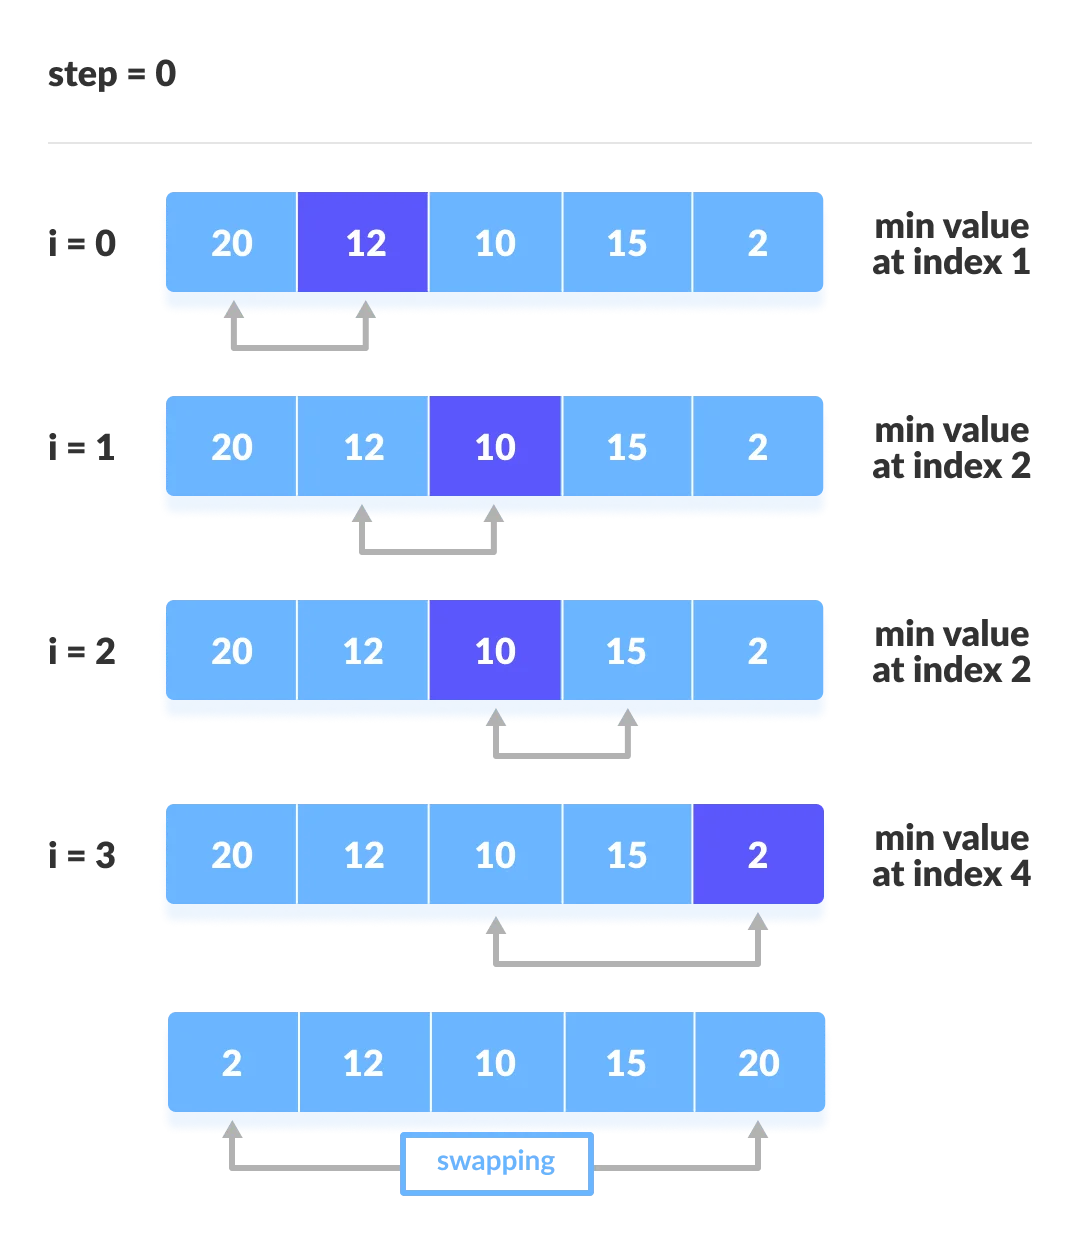
\includegraphics{Selection-sort-0}}
\end{center}
\end{frame}

\begin{frame}{Grafické znázornění 2}
\begin{center}
\scalebox{0.15}{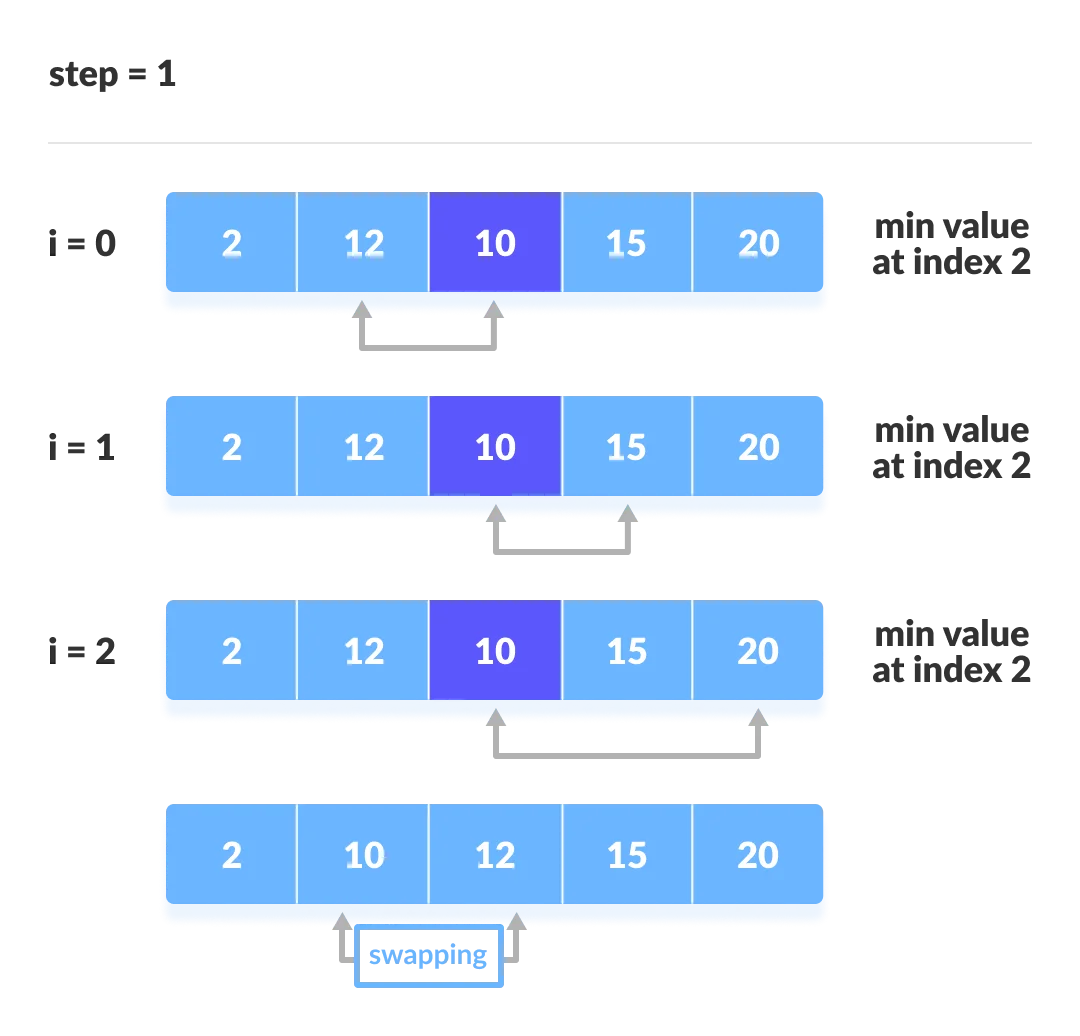
\includegraphics{Selection-sort-1.png}}
\end{center}
\end{frame}

\begin{frame}{Grafické znázornění 3}
\begin{center}
\scalebox{0.15}{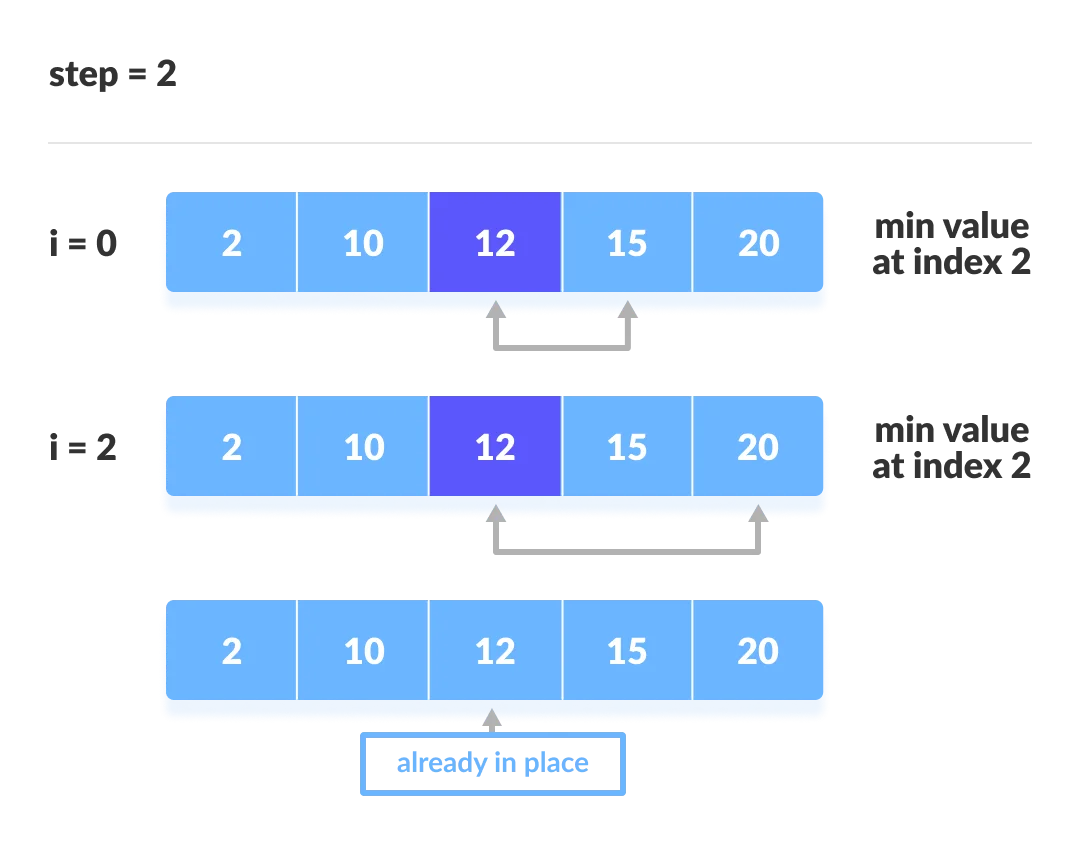
\includegraphics{Selection-sort-2.png}}
\end{center}
\end{frame}

\begin{frame}{Grafické znázornění 4}
\begin{center}
\scalebox{0.15}{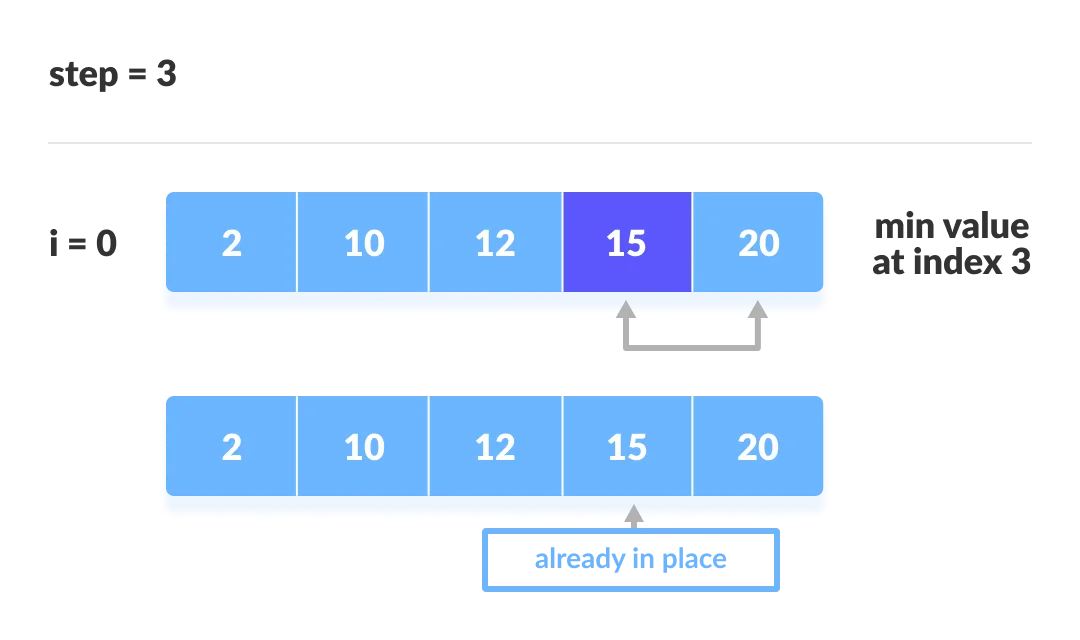
\includegraphics{Selection-sort-3_1.png}}
\end{center}
\end{frame}


\begin{frame}{Složitost}
\begin{itemize}
\item výběr nejmenšího prvku zabere průchod $n$ prvky a před výměnou prvků je tedy provedeno $n-1$ porovnání, výběr dalšího nejmenšího prvku vyžaduje průchod už jen $n-1$ prvky
\item \onslide<2->{obecně tedy v $i$-tém průchodu procházíme $n-i+1$ prvky}
\item \onslide<3->{matematicky můžeme složitost vyjádřit následovně: \[\sum_{i=1}^{n-1} i=\frac{(n-1)+1}{2}(n-1) = \frac{1}{2}(n^2-n),\]
což odpovídá složitosti $O(n^2)$}
\end{itemize}
\end{frame}

\begin{frame}{Zdroje}
\begin{itemize}
    \item Selection sort - Wikipedia [online]\\
    \url{https://en.wikipedia.org/wiki/Selection_sort}
    \item Průvodce labyrintem algoritmů [online]\\
    \url{https://knihy.nic.cz/files/edice/pruvodce_labyrintem_algoritmu.pdf}
    \item Selection Sort (With Code in Python/C++/Java/C). Programiz: Learn to Code for Free [online]\\
    \url{https://www.programiz.com/dsa/selection-sort}
\end{itemize}
\end{frame}
\end{document}
